\section{Applications}
\label{sec:apps}

In the previous sections, we described the goals of various applications
and motivated why it was difficult to accommodate them in the standard
web architecture.  Then, we described the \sys{} system, explaining the
primitives we introduced to the browser.  In this section, we close the
loop, explaining how to use this primitives to implement the
applications described in the first section.

\subsection{Encrypted Document Editor}

In the previous section, we described the key feature needed by an
encrypted document editor: symmetric confinement, where two mutually
distrusting scripts can confine each other's use of data that has been
sent.  The key to implementing this application will be judicious use of
\emph{privileges}, which are asymmetrically distributed to the
distrusting components.

\begin{figure}
\centerline{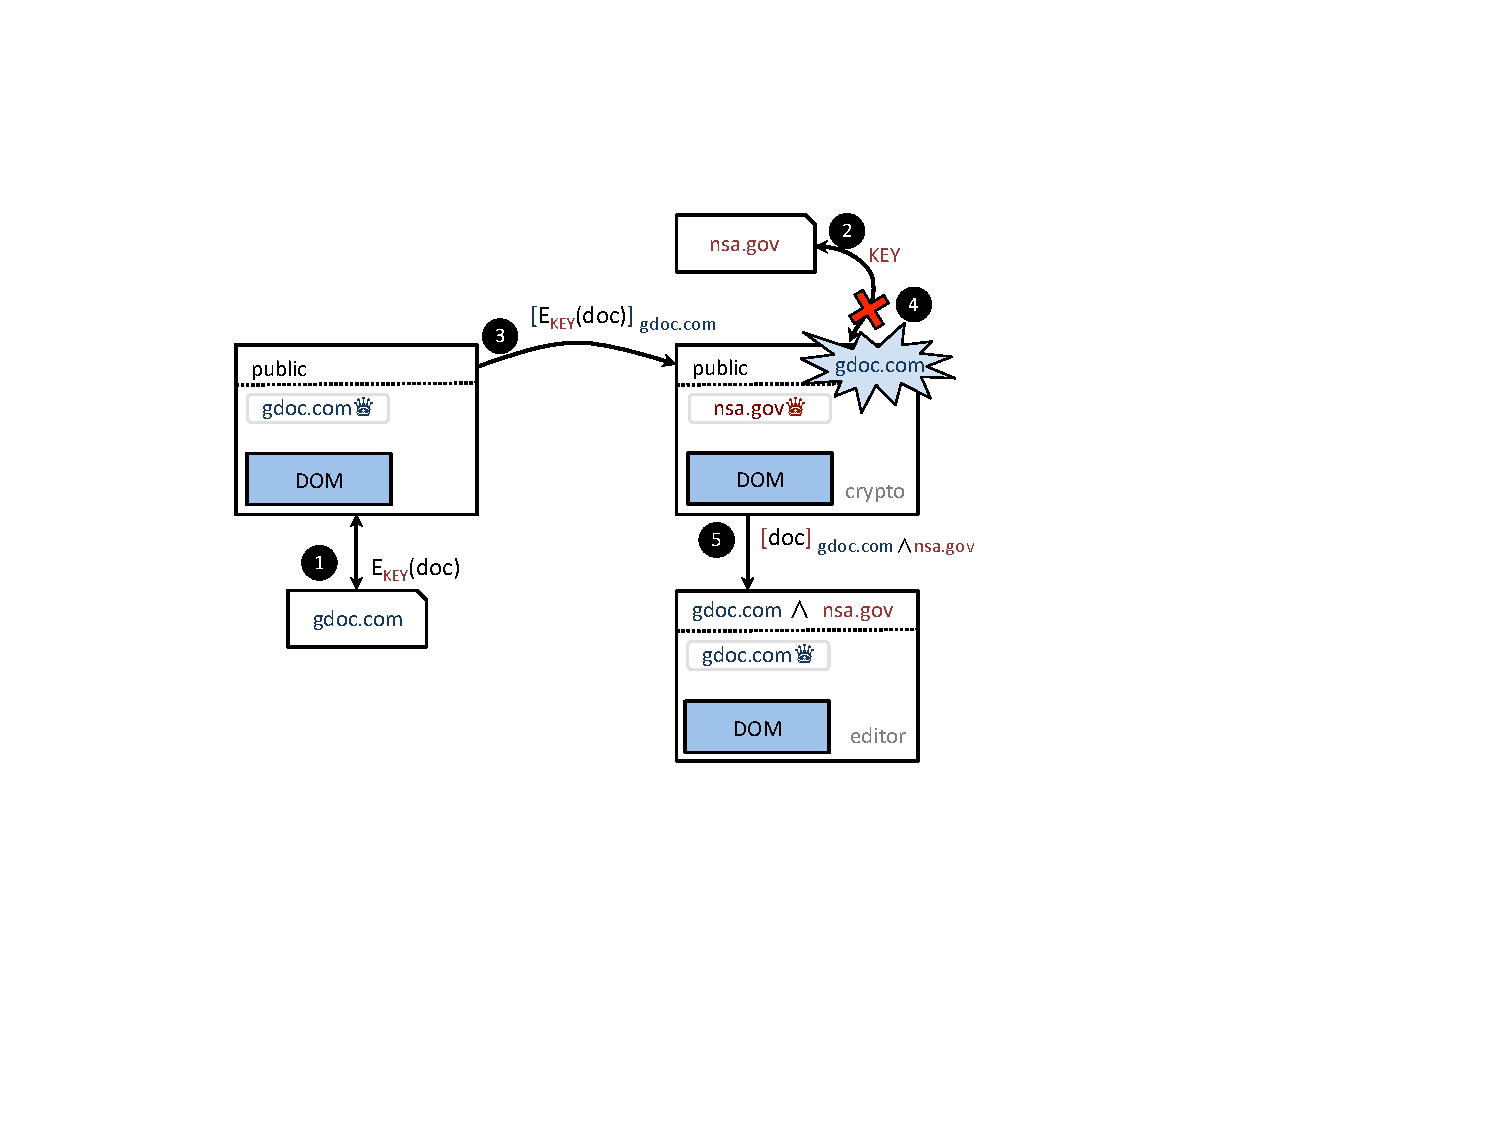
\includegraphics[width=\columnwidth]{editor}}
\caption{\label{fig:editor} Encrypted document editor architecture.}
\end{figure}

In Figure~\ref{fig:editor}, the architecture for an encrypted document
editor is shown.  The editor has three components: a component which has
your Google Documents credentials and communicates with the server (\https{gdoc.com}), the
editor proper (also \https{gdoc.com}), and the component which performs encryption (\https{nsa.gov}).  We give the
following security guarantee: if the \https{nsa.gov} is honest, then we
guarantee that the clear text of your document is never leaked to any
origin.  If only \https{gdoc.com} is honest, then \https{gdoc.com} may
be able to recover your cleartext (e.g.\ the encryptor used the null
cipher), but the encryptor should not able to exfiltrate the cleartext
to anyone else.

What occurs when you open Google Documents to edit an encrypted
document?
%
Initially, \https{gdoc.com} downloads (1) the encrypted document from
Google's servers.
%
Seeing that the document is encrypted, it opens an iframe to
\https{nsa.gov}, with initial label 
public so it can communicate with the \https{nsa.gov} server and
download the private key (2) which will be used to decrypt the document.
%
Next, it sends the encrypted document as a labeled Blob, with the label
\dcLabelS{\https{gdoc.com}}{} (3); the iframe unlabels the Blob and
raises its label (4) so it can decrypt the document.
%
Finally, the iframe passes on the decrypted document (labeled as
\dcLabelS{\https{gdoc.com} $\land$ \https{nsa.gov}}{}) to a new iframe (5) which
implements the editor proper.

To save the document, we run this flow in reverse: the editor sends a
decrypted document to the encryptor (5), which encrypts it with the
private key.  Next, the critical step occurs: the encryptor exercises its privileges
to send a labeled blob of the encrypted document which is \emph{only}
labeled \dcLabelS{\https{gdoc.com}}{} (3).  Since the encryptor is the only compartment
with the \https{nsa.gov} privilege, all documents must pass through it for
encryption before being sent out to the world; conversely, it itself cannot
exfiltrate any data, as it is operating with \https{gdoc.com} in its label.

One interesting thing to note about this architecture is that a user can
verify that Google Documents appropriately loaded the encryptor, since
without it, it would not be possible to display the decrypted text.  However, when
a new document is being created, the encryptor iframe must be placed
in a separate pop-up window, so that the user can verify that encryption
has been enabled.\footnote{This architecture might be desirable in any case
to prevent phishing.}

Due to space limitations, we do not discuss the architecture of a \sys{} 
password manager we built; this application allows users to safely store their
passwords on third-party storage provides such GoogleDocs. We only remark that
it operates on very similar principles to the encrypted document editor.

\subsection{Third-Party Mashup}
\label{sec:apps-mashup}

\begin{figure}
\centerline{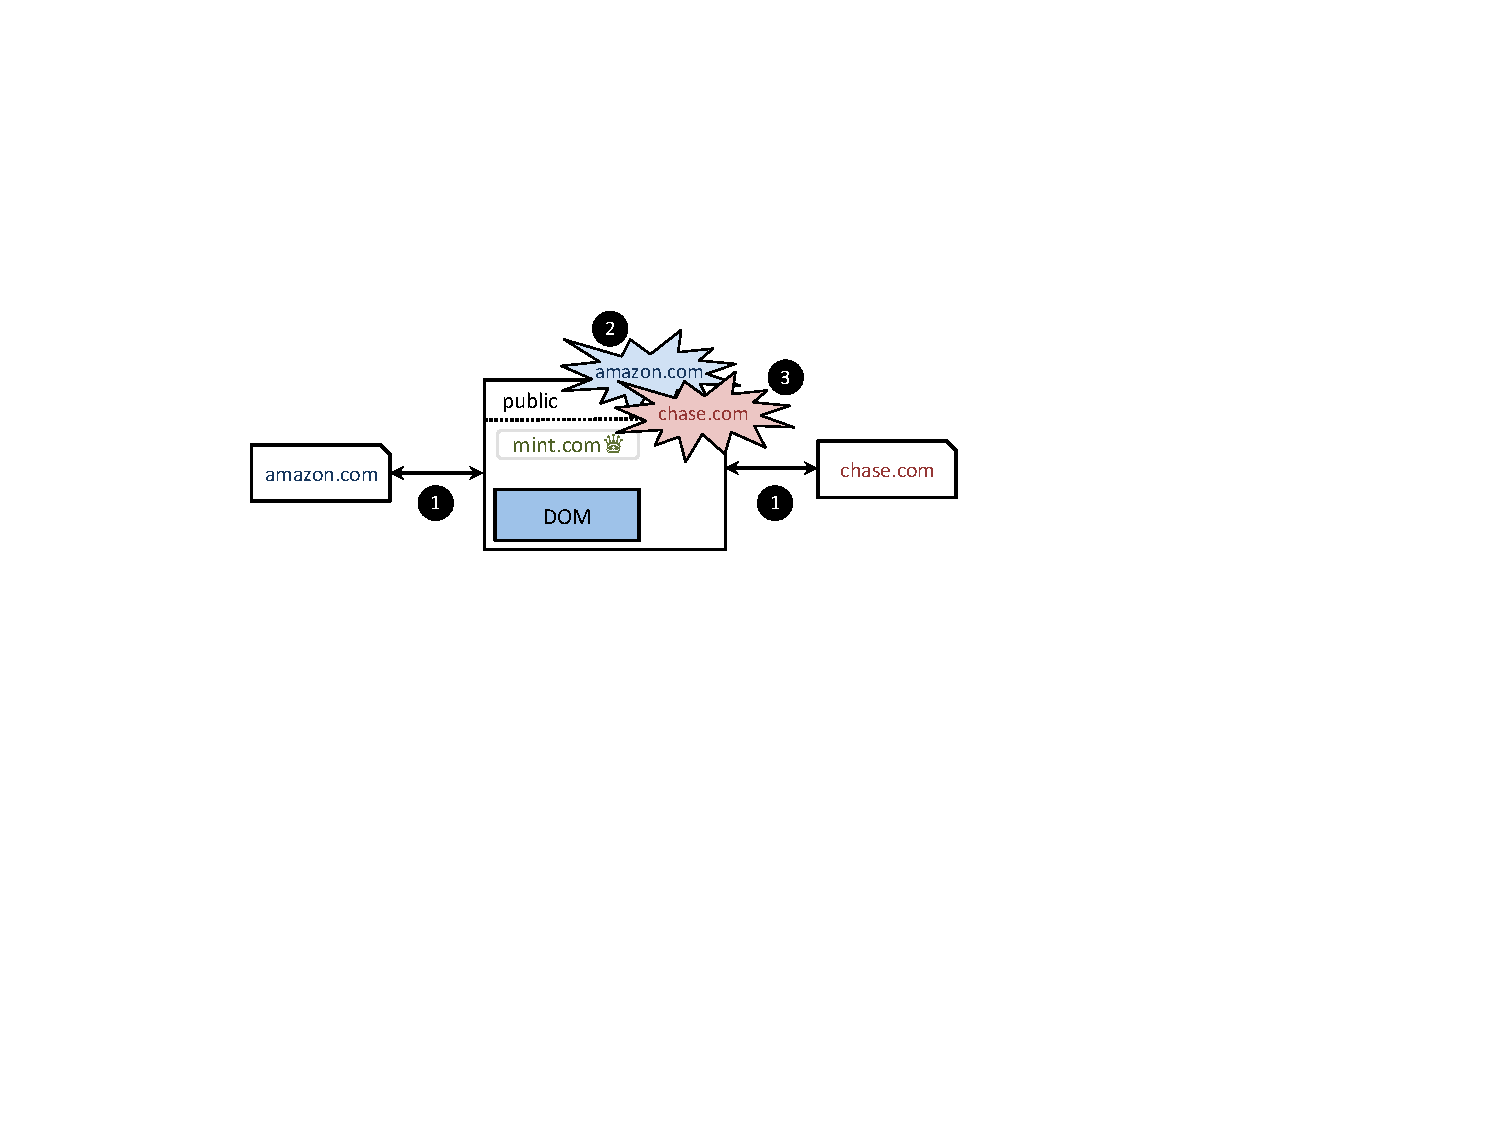
\includegraphics[width=\columnwidth]{mashup}}
\caption{\label{fig:mashup} Third-party mashup under \sys{}.}
\end{figure}
The key feature that enables us to build third-party mashups is
labeled XHR, as it composes with CORS.
%
Today's CORS policies are DAC-only, such that a server must
either allow another origin to read its data, and fully trust that
origin not to disclose the data, or deny the other origin access to
the data altogether. Under COWL, however, a server could
CORS-whitelist a foreign origin to permit that origin to read its
data, and by setting a label on its response, be safe in the knowledge
that COWL would appropriately confine the foreign origin's scripts in
the browser.
 
In Figure~\ref{fig:mashup},
the architecture for an application which reconciles a user's Amazon
purchases and bank statement is shown. 
%
Here, Chase and Amazon respectively expose (read-only) bank statement,
and purchase history APIs that whitelist known applications' origins,
such as \https{mint.com}, but set MAC labels on responses.
%
(As discussed in Section~\ref{sec:discussion}, with MAC in place, COWL
allows users to otherwise augment CORS by whitelisting cross-origins
on a per-origin basis.)
%
% The rest is very simple.
%
Using labeled XHR, we make requests to both web sites (1),
to receive the bank statement and
purchase history as labeled Blobs.
%
Once all of the information is received, we unlabel it and raise
our context label accordingly (2--3); this restricts our communication
to the web at large.

We remark that, in contrast to solely using CORS, by setting by MAC
labels on responses, Chase and Amazon need not trust Mint to write
bug-free code---COWL confines the Mint code to ensure that it cannot
arbitrarily leak bank statements or purchase histories. As we discuss
in Section~\ref{sec:discussion}, however, a malicious Mint application
could potentially leak data through covert channels.  We emphasize
that COWL nevertheless offers a significant improvement over the
status quo, in which, \emph{e.g.,} users give their login credentials to
Mint, and thus not only trust Mint to keep their bank statements
confidential, but also not to steal their funds!

\subsection{Untrusted Third-Party Library}
\label{sec:apps-third-party}

\begin{figure}
\centerline{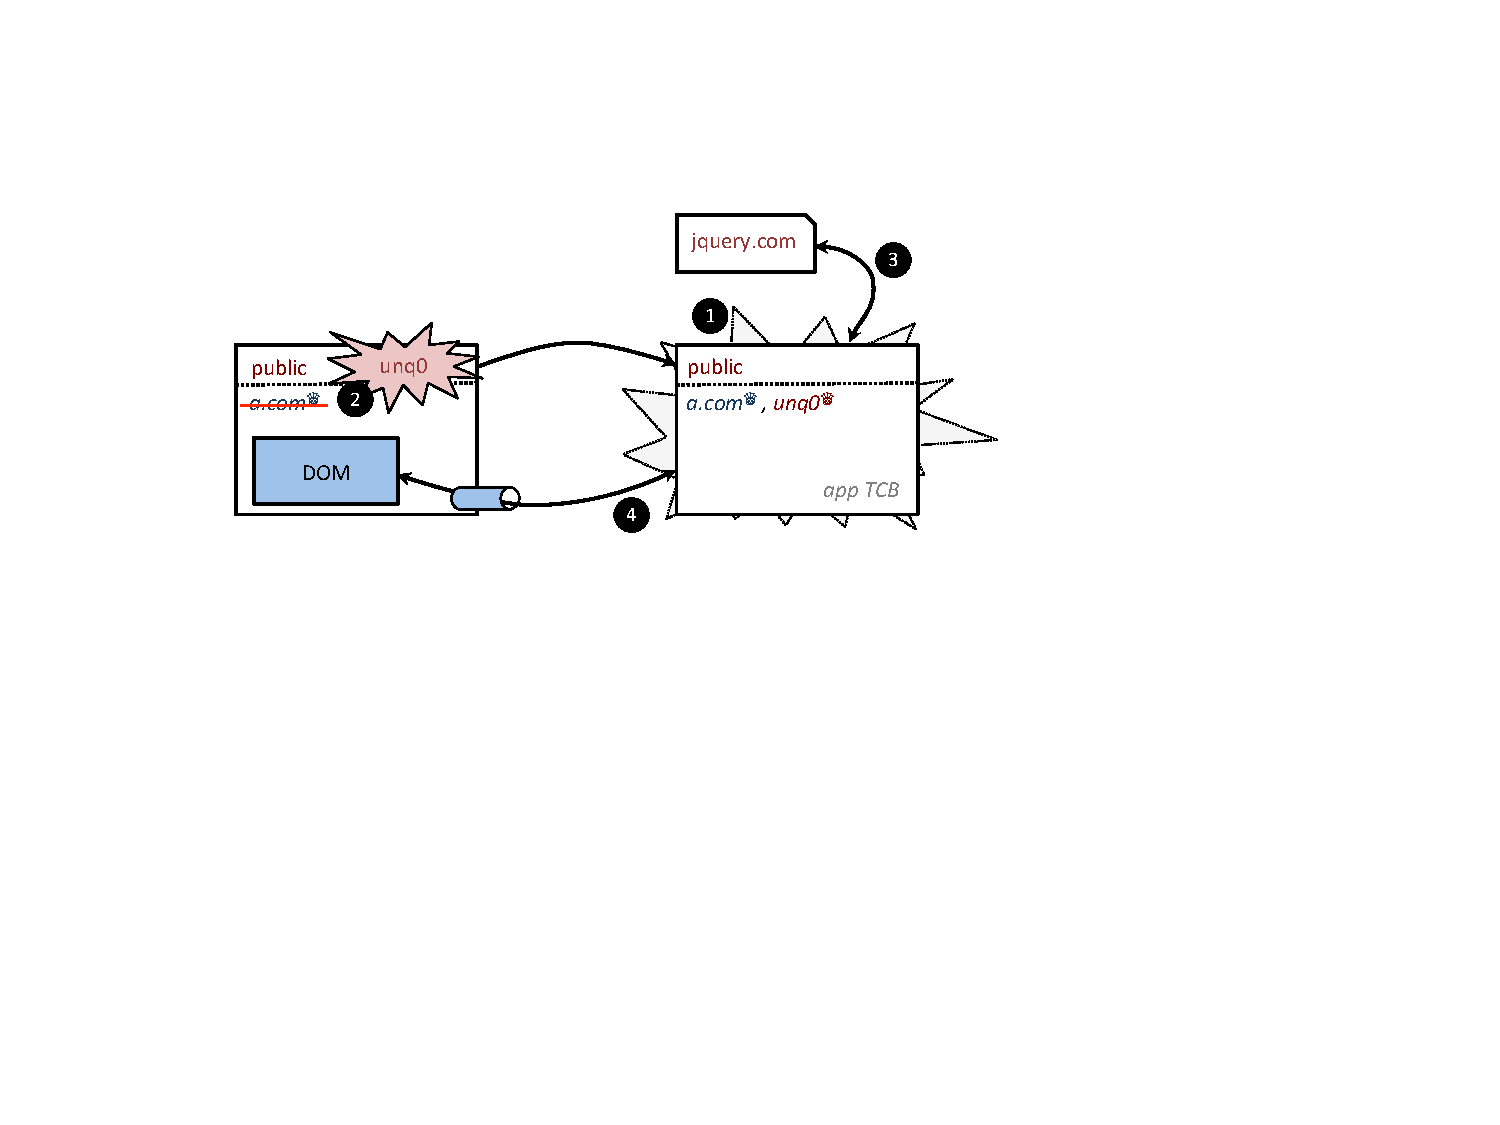
\includegraphics[width=\columnwidth]{jquery}}
\caption{\label{fig:jquery} Privilege separation and library
confinement.}
\end{figure}

The key features that let us confine tightly-couple untrusted
third-party libraries like jQuery is the ability to delegate
privileges to a trusted context and subsequently drop them from the
main page. In doing so we can completely confine the main page, and
ensure that it can only communicate with the trusted and unconstrained
context.

In Figure~\ref{fig:jquery}, the architecture for a web page using an
untrusted JavaScript library is shown.  Our goal is to establish a
separate DOM worker which has the \https{a.com} privilege, while the
main browsing context runs jQuery without privileges or the ability to
talk to the network.  Initially, we start in the main browsing context
with the \https{a.com} privilege.  We generate a fresh origin
\https{unq0}, and spawn a DOM worker (1), delegating it both privileges.  The
main context then drops its privileges and raises its label to
\dcLabelS{\https{unq0}}{} (2).  Finally, the
trusted worker downloads jQuery (3) and injects the script contents
into to the main context's DOM (4).  At the time the library
is loaded, the main context becomes untrusted, but this is no matter, as
it is fully confined at this point.  As the trusted DOM worker has both
privileges, it can freely modify the DOM of the main context, as well as
communicate with the wider web.  We can think of this DOM worker as a
\emph{firewall} between the page proper (with the untrusted library)
and the rest of the world.
